% !TeX spellcheck = en_GB
\documentclass[10pt,letterpaper,oneside]{article}
\usepackage{fontspec}
\usepackage{arev}
\usepackage[utf8]{inputenc}
\usepackage[T1]{fontenc}
\usepackage{amsmath}
\usepackage{amsfonts}
\usepackage{amssymb}
\usepackage{graphicx}
\usepackage{csquotes}
\usepackage{booktabs}
\usepackage{multicol}
\usepackage{enumerate}
\usepackage{microtype}
\usepackage[labelfont=bf,font={small}]{caption}
\usepackage{hyperref}
\usepackage{booktabs}
\usepackage{subcaption}
\usepackage{fancyhdr}
\usepackage[svgnames]{xcolor}
\usepackage{mdframed}
\usepackage{multicol}
\usepackage[para]{footmisc}
\usepackage{siunitx}
\usepackage{cleveref}
\usepackage{listings}
\usepackage{cprotect}


\lstset{ % General setup for the package
	language=Python,
	basicstyle=\small\ttfamily,
	tabsize=4,
	columns=fixed,
	showstringspaces=false,
	showtabs=false,
	keepspaces,
	commentstyle=\color{SeaGreen},
	keywordstyle=\bf\ttfamily\color{DarkBlue}
}

\newfontfamily\symbolfont{Symbola}
\usepackage[left=1in,right=1in,top=1in,bottom=1in,marginparwidth=0.3in]{geometry}

\usepackage[sorting=none]{biblatex}
\addbibresource{../bibliography.bib}

\author{Andreas Stöckel\\[0.5cm]Based on lecture notes by\\Chris Eliasmith and Terrence~C.~Stewart}
\newcommand{\baseCodeURL}{https://github.com/astoeckel/syde556-w20/blob/master/lectures}

\fancyhf{}
\fancyhead[L]{SYDE 556/750 Lecture Notes}
\fancyhead[R]{Andreas Stöckel}
\fancyfoot[C]{\thepage}
\pagestyle{fancy}

\setlength{\parindent}{0em}
\setlength{\parskip}{0.5em}
\renewcommand{\baselinestretch}{1.25}
\renewcommand{\vec}[1]{{\mathbf{#1}}}
\newcommand{\mat}[1]{{\mathbf{#1}}}
\newcommand{\T}{\ensuremath{\mathrm{T}}}
\renewcommand{\epsilon}{\varepsilon}
\renewcommand{\phi}{\varphi}

\makeatletter
\newcommand{\superimpose}[2]{%
	{\ooalign{{#1}\hidewidth\cr{#2}\hidewidth\cr}}}
\makeatother
\newcommand{\SolidCircle}[2]{\superimpose{\color{#1}\symbolfont ⬤}{\textbf{\color{white}#2}}\hspace{1em}}
\newcommand{\OPlus}{\SolidCircle{DarkGreen}{\kern0.75pt+}}
\newcommand{\OMeh}{\SolidCircle{DarkOrange}{~}}
\newcommand{\OMinus}{\SolidCircle{DarkRed}{\kern2.25pt--}}

\newcommand{\YouTube}[2][Video]{\href{https://youtu.be/#2}{{\symbolfont 📺}~{#1}}%
%\footnote{\url{https://youtu.be/#2}}%
}

\newcommand{\CodeLink}[2][Code]{\href{\baseCodeURL/#2}{{\symbolfont ⌨}~\emph{#1}}}

\newcommand{\MakeTitle}[1]{
\maketitle
\begin{center}
	
\includegraphics[width=0.5\textwidth]{../assets/uwlogo.pdf}\\[1cm]
	{#1}\
\end{center}

\vfill

\thispagestyle{empty}
\setcounter{page}{0}
\newpage

\pagenumbering{roman}
\setcounter{tocdepth}{2}
\tableofcontents
\newpage

\setcounter{page}{0}
\pagenumbering{arabic}}

\reversemarginpar


\newcommand{\ColorBox}[3]{%
	\marginpar{%
		\huge\raisebox{-3ex}{\symbolfont{#1}}%
	}%
	\begin{mdframed}[hidealllines=true,backgroundcolor=#2,innertopmargin=0.25cm,innerbottommargin=0.25cm]%
		{#3}
	\end{mdframed}}

\newcommand{\Note}[1]{\ColorBox{📌}{WhiteSmoke}{\textbf{Note:} #1}}
\newcommand{\Example}[1]{\ColorBox{💡}{WhiteSmoke}{\textbf{Example:} #1}}
\newcommand{\Aside}[1]{\ColorBox{🌟}{WhiteSmoke}{\emph{Aside:} #1}}
\newcommand{\Python}[1]{\ColorBox{🐍}{WhiteSmoke}{#1}}
\newcommand{\Notation}[1]{\ColorBox{\huge$\Sigma$}{WhiteSmoke}{\textbf{Notaton:} #1}}

\newcommand{\ConstructionSite}{\hrulefill {\symbolfont 🚧} UNDER CONSTRUCTION {\symbolfont 🚧} \hrulefill}

\newenvironment{ImportantEqn}[1]{\mdframed\raggedleft\emph{({#1})}\align}{\endalign\endmdframed}

\date{January 7, 2020}
\title{SYDE 556/750 \\ Simulating Neurobiological Systems \\ Lecture 1: Introduction}


\begin{document}

\MakeTitle{\textbf{Accompanying Readings: Chapter 1 of Neural Engineering}}

\section{Overview}

\Note{This entire lecture is meant to give you a broad, whirlwind overview of the material in the course. We're going to revisit most of the topics mentioned here in much more detail in the upcoming weeks.}

\subsection{Overall Goal of This Course}

The overall goal of this course is to explore methods for modeling and simulating large-scale neurobiological systems. By large-scale we mean that we're focusing on the properties of nervous \emph{systems} and less on the interaction between their individual components (i.e., individual neurons).

Put differently, our goal is to systematize the construction of brain models -- or at least the constructions of models of brain subsystems.

So, beyond the \emph{obvious} fact that building brain models is the most interesting thing in the world, why should you be excited about this course? What are potential applications of the material we're going to discuss?
\begin{enumerate}[1.]
	\item \textbf{Figuring out how the brain works}
	\begin{itemize}
		\item Health applications (better treatment of diseases).
		\item Philosophical implications (new ways of understanding the mind and who we are).
	\end{itemize}
	\item \textbf{Building better AI systems}
	\begin{itemize}
		\item Understanding how the brain works may help us to build better AI systems.
		\item \enquote{Classical AI} (structured; symbolic) $\leftrightarrow$ \enquote{Deep Learning} (unstructured, \enquote{sub-symbolic}, grounded). We're discussing solutions that are somewhere in between, i.e., systems that are structured but still able to learn with symbol grounding.
	\end{itemize}
	\item \textbf{Programming neuromorphic hardware}
	\begin{itemize}
		\item (Spiking) neuromorphic hardware systems are inspired by brain like-information processing. The methods we discuss in this course facilitate programming this hardware.
	\end{itemize}
\end{enumerate}

\subsection{Theoretical Neuroscience}

\begin{figure}
	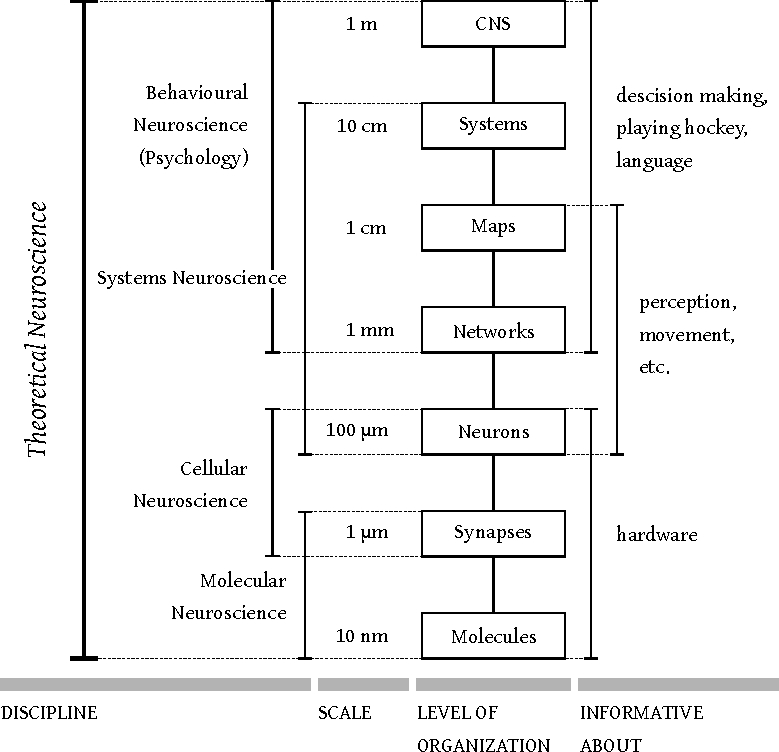
\includegraphics{media/levels.pdf}\\
	\caption{Levels of Organization. Adapted from ???.}
	\label{fig:levels}
\end{figure}

\begin{itemize}
	\item How does the mind work?
	\item Most complex and most interesting system humanity has ever studied Why study anything else?
	\item How should we go about studying it?
	\begin{itemize}
		\item What techniques/tools?
		\item How do we know if we're making progress?
		\item How do we deal with the complexity?
	\end{itemize}
\end{itemize}

\newpage

\subsection{A Useful Analogy}

{\centering
	\begin{tabular}{p{4cm} p{4cm} p{4cm}}
		\toprule
								  &
								  \textbf{Theoretical physics} & \textbf{Theoretical\newline neuroscience} \\
		\midrule
		\raggedright\emph{Quantify} phenomena & $\vec{F} = m \vec{a}$ & $\hat{\vec x} = \mat D \vec a$ \\
		\midrule
		\raggedright Summarize lots of data & motion of objects & neural representation of information \\
		\midrule
		\raggedright Speculative (generate hypotheses) & true for all velocities & true for all stimuli \\
		\bottomrule
	\end{tabular}\\\textbf{Table:} Comparison between theoretical physics and theoretical neuroscience. Adapted from ???}

\begin{itemize}
	\item What is Theoretical Neuroscience?
	\item A useful analogy is to theoretical physics
	\begin{itemize}
		\item Similarities
		\begin{itemize}
			\item Methods are similar
			\item Goals are similar (quantification)
		\end{itemize}
		\item Difference
		\begin{itemize}
			\item Central question "What exists? vs. Who are we?"
			\item More simulation (because of nonlinearities) in biology
		\end{itemize}
	\end{itemize}
\end{itemize}

\section{Neural Modelling}

\begin{itemize}
	\item Let's build it
	\begin{itemize}
		\item Specify theory in enough detail that this is possible
		\item Tends to get complex, so need computer simulation
	\end{itemize}
	\item Bring together levels and modeling methods
	\begin{itemize}
		\item Single neuron models (levels of detail; e.g. spikes, spatial structure, various ion channels, etc.)
		\item Small network models (levels of detail; e.g. spiking neurons, rate neurons, mean fields, etc.)
		\item Large network/cognitive models (levels of detail; e.g. biophysics, pure computation, anatomy, etc.)
		\item Ideally allow all levels of detail below any higher level to be included as desired.
		\item 'Correct' level depends on questions being asked.
	\end{itemize}
\end{itemize}

\subsection{Problems with current approaches}

\paragraph{Large-scale neural models (e.g. Human Brain Project, Synapse Project, etc.)}

\begin{itemize}
	\item Lack of function or behaviour
	\begin{itemize}
		\item Can't compare to psychological data
	\end{itemize}
	\item Assumes canonical algorithm repeats
	\begin{itemize}
		\item e.g., Measurements from one small part (hippocampus) are valid everywhere
		\item But, different parts of the brain are very different (connectivity, cell types, inputs/outputs)
	\end{itemize}
	\item Expects intelligence to 'emerge'
	\begin{itemize}
		\item Unclear what 'emergence' means, how it will work, or what it explains
		\item Wishful thinking?
	\end{itemize}
\end{itemize}

\paragraph{Cognitve models (e.g. ACT-R, Soar, etc.)}

\begin{itemize}
	\item Disconnected from neuroscience, can't compare to neural data
	\begin{itemize}
		\item Trying to map components of the model to brain areas
		\item When a component is active, maybe neurons in that area are more active?
	\end{itemize}
	\item No "bridging laws"
	\begin{itemize}
		\item Like having rules of chemistry that never mention that it's all built out of atoms and electrons
	\end{itemize}
	\item No constraints on the equations
	\begin{itemize}
		\item Just anything that can be written down
		\item Many possibilities; hard to figure out what matches human data best
	\end{itemize}
	\item Maybe that's okay
	\begin{itemize}
		\item Do we understand the brain enough to make this connection and constrain theories?
		\item When understanding a word processor, do we worry about transistors?
	\end{itemize}
\end{itemize}

\section{The Brain}

\begin{itemize}
	\item 2 kg (2\% of body weight)
	\item 20 Watts (25\% of power consumption)
	\item Area: 4 sheets of paper
	\item Neurons: 100 billion $10^{11}$ ($15\,0000$ per $mm^2$)
	\item Synapses: at least 100 trillion $10^{14}$ (about $1000$-$10000$ per neuron)
\end{itemize}

\section{Brain structures}


\section{The Neural Engineering Framework and the Semantic Pointer Architecture}

Now that we've spent some time discussing other approaches aiming at large-scale modelling of neurobiological systems and pointing out their shortcomings, what is the approach at neural modelling, we're going to discuss in this course? Actually, we're going to have a look at two different modelling techniques: the \emph{Neural Engineering Framework}, and the \emph{Semantic Pointer Architecture}.

\subsection{Neural Engineering Framework}
The \emph{Neural Engineering Framework} (NEF) has been proposed by Eliasmith and Anderson in their book \enquote{Neural Engineering} in 2003 \cite{eliasmith2003neural}. We will spend about two thirds of this course on discussing the NEF.

The goal of the Neural Engineering framework is to treat the brain as a purely physical system and to use techniques form engineering -- such as control theory, information theory, and signal processing theory -- to aid a \emph{functional} understanding of the brain in theoretical neuroscience. After all, building physical systems that perform a certain function and -- to this end -- \emph{understanding} physical systems in terms of their potential function lies at the heart of engineering practice.\footnote{This is akin to Richard Feynman's famous chalkboard note \enquote{What I cannot create, I do not understand.} \cite{richard1988richard}} Of course, a major difference lies in the fundamental components usually employed by nature and, conversely, be engineers. Natural systems have evolved, and their individual parts, such as neurons, are thus inherently diverse and \enquote{messy}. Engineers on the other hand often rely on precisely manufactured parts. So when applying engineering methods to neural modelling, we somehow have to take this messiness into account. As we will see later, we can actually use the \enquote{messiness} of neural systems to our advantage when building models.

The Neural Engineering Framework provides a systematic way to translate a vector-valued dynamical system into a spiking neural network. In other words, the NEF can be thought of as a \emph{neural compiler}, that turns a mathematical description into a spiking neural network. Most importantly, this translation process can be informed by the vast corpus of neuroscientific data collected over the past decades. To put it differently: given a mathematical model, and a set of neurobiological constraints, including neural tuning, neuron count, connectivity, and time constants, we can create a neural network that fulfils these constraints and approximates the mathematical model.

\subsection{Semantic Pointer Architecture}
The second technique---which we're going to discuss during the last third of the course---is the \emph{Semantic Pointer Architecture} (SPA). The SPA is a mathematical tool for building models of high level cognition. It is based on what's commonly referred to as a \emph{Vector Symbolic Architecture} (VSA) and has been described in the book \emph{How to Build a Brain} by Eliasmith published in 2013 \cite{eliasmith2013how}.

VSAs provide a way to implement discrete symbolic architectures as they have been used in classical aritficial intelligence research (\enquote{Good Old Fashioned AI}; GOFAI) on top of continuous vector spaces. The SPA in particular describes how such \enquote{symbol vectors}, also called \enquote{semantic pointers}, can be generated from sensory input, combined---or bound to---other semantic pointers, and decompressed back into either the sensory or motor domain.

\subsection{The NEF and SPA as a tool for hypothesis generation}
While the NEF and SPA are independent concepts, they can be combined into a powerful tool for scientific exploration in theoretical neuroscience. In particular, the NEF provides a way to represent vector spaces on a neural substrate, and, conversely, the SPA provides a way to implement a cognitive architecture on top of vector spaces. In other words, the NEF describes the computational substrate, whereas the SPA can make use---but is not limited to---this substrate. This means that we have a powerful tool at our disposal which -- looking back at \cref{fig:levels} -- can be used to model biological systems from modelling synapses and neurons up to entire central nervous systems.

Of course, merely using these techniques does not magically mean that the models we build with them are good models of human cognition. In fact, depending on the kind of question we're trying to answer, our models are most definitively wrong, but that is the nature of models. The true strength of the NEF and the SPA is in aiding \emph{hypothesis generation}.

For example, we might have an hypothesis as for how a certain cognitive task could be solved nn terms of the SPA. We furthermore know from empirical research which brain regions in are involved in solving this task, and as such have data from neuroscience. We can now use this data as constraints when mapping the model onto the brain using the NEF. The resulting spiking neural network model can then be simulated and probed in various ways. This allows us \emph{(a)} to \emph{verify} our hypothesis by comparing high-level behaviour data (e.g.,~timings and error rates) between human/animal subjects and our model and \emph{(b)} to make \emph{predictions} about what we should be able to measure in the case of experiments that have not been performed on real subjects.

\subsection{The Nengo Simulator}
In the end, the NEF and the SPA are just mathematical concepts. In order to aid scientists in pursuing the kind of hypothesis-driven research outlined above, we need tools that facilitate the construction of such models. The \enquote{\texttt{nengo}} (originally short for \enquote{\emph{N}eural \emph{Eng}ineering \emph{O}bjects}) neural network simulation package is such a tool. It not only provides convenient interfaces for building NEF and SPA models (as well as other kinds of artificial neural networks), but can also execute the resulting model on a variety of hard- and software-backends such GPUs and analogue and digital neuromorphic hardware.

\texttt{nengo} was originally developed by members of the Computational Neuroscience Research Group (CNRG) at the University of Waterloo \cite{bekolay2014nengo}. It is now developed by a company called ABR (Applied Brain Research). \texttt{nengo} is available free-of-charge for non-commercial use. It can be found at \url{https://nengo.ai} and \url{https://github.com/nengo}.

\Note{As part of the assignments we're going to write our own software implementation of the NEF. Correspondingly, for the sake of learning the underlying theory, you cannot use \texttt{nengo} at first. However, you are asked to use \texttt{nengo} for the last assignment, and are free to use it for the final project. So it definitively doesn't hurt to have a look at it.}

\section{Noise, Representation, Transformation, and Dynamics}

The Neural Engineering Framework is based on three principles: Representation, Transformation, and Dynamics. We will have a closer look at each of these principles in upcoming lectures, but for now, let's quickly summarize what each of these principles is about.

\subsection{Representation}

In order to solve complex tasks, nervous systems must construct \emph{representations} of their environment. A reasonable definition of \emph{representation} would be to say that a neuron \emph{represents} some aspect of the environment, if this neuron is active (or conversely, exactly not active) whenever a certain stimulus is present. In other words, if there is a causal relationship between the stimulus and the neural activity. However, in general, the question of how exactly neurons represent information is still open.

In accordance with the above, we think of representations in the NEF as the mapping between a \emph{value} that is being processed in the network and the corresponding \emph{activity} of a \emph{group} of neurons. Mathematically speaking, the neural activity can be seen as a vector $\vec a(t)$ in a high-dimensional vector space, whereas the corresponding value $\vec x(t)$ may be a situated in a lower-dimensional vector space.

For this concept of representation to be useful, we need to define a way to \emph{decode} the represented value from the neural activity, and also a way to \emph{encode} a value as neural activites. The NEF defines the decoding process in terms of a linear decoder, and the encoding process in terms of a nonlinear encoding.

Note that we talked representations in terms of the activity of a \emph{population} -- also referred to as an \emph{ensemble} -- of neurons, and not in terms of the activity of individual neurons. This is an important difference that separates the NEF from many \enquote{classical} modelling approaches in neuroscience. The NEF focuses on neuron populations as the smallest representational unit, and not individual neurons.

\Example{Famous examples of neural representation are place- and grid-cells. Here neural activity is correlated with the animal being a certain location (place cells,~\cite{okeefe1978hippocampus}), or within a certain patch of a multi-scale hexagon grid (grid cells,~\cite{hafting2005microstructure}, see \cref{fig:hafting_et_al_2005_grid_cells}).  We're going to revisit grid cells when we talk about spatial semantic pointers. Another, more classical example is orientation tuning in primary visual cortex. Here, cells represent the orientation of line-shaped features in the visual field. See \cref{fig:eliasmith_et_al_2003_orientation_tuning}.}

\begin{figure}[t]
	\begin{subfigure}[b]{0.5\columnwidth}
		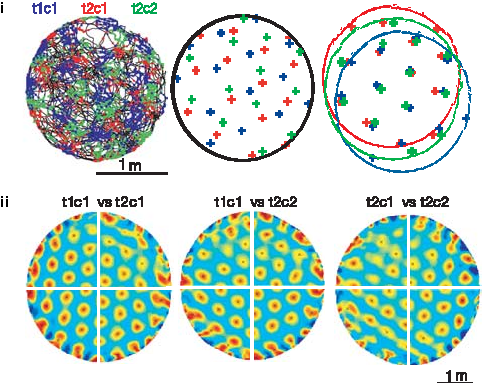
\includegraphics[width=\columnwidth]{media/hafting_et_al_2005_grid_cells.pdf}
		\caption{Grid cells}
		\label{fig:hafting_et_al_2005_grid_cells}
	\end{subfigure}
	\begin{subfigure}[b]{0.5\columnwidth}
		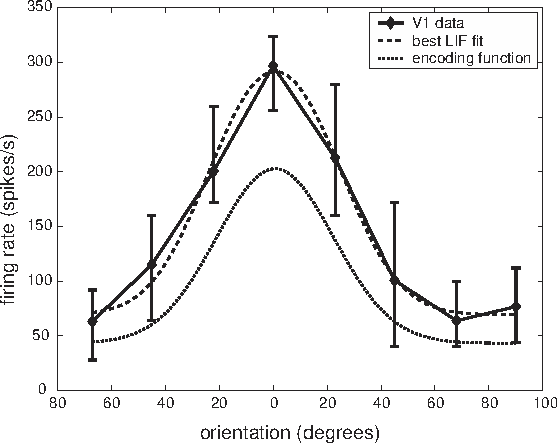
\includegraphics[width=\columnwidth]{media/eliasmith_et_al_2003_orientation_tuning.pdf}
		\caption{Visual orientation tuning}
		\label{fig:eliasmith_et_al_2003_orientation_tuning}
	\end{subfigure}
	\caption{\textbf{Examples of neural representation.} \textbf{(a)} Grid cells. Top left: trajectory of the experimental animal while moving through space. Colours (ref, blue, green) correspond to the activity of three cells recorded from the dorsocaudal medial entorhinal cortex (dMEC). Top centre: peak activity locations for each cell. Top right: the individual cell peak activities are shifted to coincide with each other, highlighting the repeating structure in each cell. Bottom: cross-correlations between the individual cell activities. Figure copied from \cite{hafting2005microstructure}, fig.~3. \textbf{(b)} Example of visual orientation tuning of a cell in primary visual cortex of a macaque monkey. Figure copied from \cite{eliasmith2003neural}, fig.~3.1.}
\end{figure}

\Note{When talking about representations in this course, we generally refer to \enquote{transient} activities of the network, i.e.,~relatively short-lived signals. Of course, longer-lived states -- such as \emph{long-term memories} -- are also represented in the brain somehow, but we'll talk about this separately when discussing learning.}

\subsection{Transformation}

Of course, merely being able to represent values within biologically plausible neural networks is not sufficient to explain complex behaviours. We need some notion of computation, i.e., the ability to compute functions $f(\vec x¸)$ given a represented vectorial value $\vec x$.

Functions are being computed by choosing the right synaptic weights that connect two populations of neurons. In a sense, we could say that the \emph{connections between populations} compute functions.

\subsection{Dynamics}

%\section{Examples}git

\printbibliography

\end{document}